\documentclass[journal]{IEEEtran}

\usepackage{amsmath}
\usepackage{amssymb}
\usepackage{graphicx}
\graphicspath{{figures/}}
\usepackage{cite}
\usepackage{url}
\usepackage{float}

\hyphenation{op-tical net-works semi-conduc-tor}
\renewcommand{\arraystretch}{0.85}
\def\IEEEkeywordsname{Keywords}
\renewcommand{\figurename}{Figure}

\begin{document}

\title{Reliable Structured-Decision Applicant Ranking with a Non-Autoregressive System One Model}

\maketitle

\begin{abstract}
LLM applicant-ranking pipelines usually place the whole decision in one autoregressive model's judgment, whose free-text justification is not guaranteed to reflect what actually drove it. The research objective is to determine how much of that decision can be made without the model's most expensive judgment, tested on real data: 301 resumes against 10 real job postings. The research method builds a pipeline on Jev, TypeSafe AI's non-autoregressive, typed-decision model: Jev answers one typed Choice question per requirement, and its probability distribution is averaged into one auditable criterion score, the primary ranking signal. Candidates enter a tie cluster only within a tolerance floored at Jev's measured noise; only there does a pairwise tournament query Jev, bounded in effect. The result shows a 90.2\% candidate-job pair reduction from a local shortlist gate, a content-preserving evidence-ordering bias cut from 6.25\% to 0--1.6\% (now guaranteed by construction), and, on a full-coverage reliability pilot, 93.1\% tiering-validity agreement and 93.6\% repeat-call consistency. Full-ranking repeatability, checked at full coverage on a second job profile, \texttt{data-engineer} (66 shortlisted candidates), gives a mean Kendall's $\tau=0.981$ across three independent re-runs, with the active tournament converging within its iteration budget in every repeat. To our knowledge, this is the first applied use of a non-autoregressive, typed-decision model for candidate ranking, and the first to measure, fix, and verify its presentation-bias mitigation in production.
\end{abstract}

\begin{IEEEkeywords}
Applicant Ranking, Human Resources, Large Language Models, Non-autoregressive Model, Structured Decision.
\end{IEEEkeywords}

\IEEEpeerreviewmaketitle

\section{Introduction}

\IEEEPARstart{R}{ecruitment} platforms increasingly use large language models (LLMs) to read resumes and compare applicants against a job profile \cite{ref1,ref3,ref4}. Whatever the output format -- free text, a score, a pairwise preference -- the pattern is usually the same: one model call renders the whole judgment, with no structural way to tell a well-supported decision from a lucky one. A ranking that can shift because of a single noisy call or an arbitrary evidence order is not defensible to the person it ranked, regardless of the model's benchmark accuracy.

Given a model that returns typed answers with native confidence instead of free text, how much of a ranking decision can be made without its most expensive, holistic, and -- as this paper measures directly -- noisy comparison at all? The research objective is to build such a pipeline and report what running it end to end on real data actually shows.

Three gaps motivate this design. First: Jev, released September~15, 2026, is the first widely-documented non-autoregressive, typed-decision model -- structured input in, a probability and confidence per question out, no free text \cite{ref5,ref6,ref7}. No prior work applies Jev, or a model like it, to applicant ranking; most existing systems estimate confidence indirectly from an autoregressive judge \cite{ref1,ref3,ref4,ref10}. The paper is accordingly not a new judge but a scoring, routing, and ranking design built around a typed, probabilistic judge: a per-criterion distribution cheap enough to be the primary signal, and a holistic comparison reserved for cases that signal cannot resolve. Second, a recent 2026 audit \cite{ref22} shows that presentation changes preserving a candidate's qualifications can still flip screening decisions, but none proposes a routing design, for any judge, that bounds how far one comparison can move a rank. Third, tie-tolerance thresholds in hybrid LLM-judge designs are usually assumed rather than measured from the judge's own noise, even though \cite{ref26} shows a pairwise judge's reliability specifically degrades on near-tie pairs -- exactly the pairs such a threshold should route to the costlier signal.

This paper's contribution is threefold. (1) A scoring, routing, and ranking design built on Jev's typed interface: a probability-weighted per-criterion score is the primary signal; Jev's pairwise judgment runs only inside tie clusters floored at the judge's measured noise; the resulting adjustment is provably bounded within a cluster. To our knowledge this is the first applied use of Jev, or any non-autoregressive typed-decision model, for candidate ranking. (2) Empirical validation on 301 real resumes against 10 real job postings: a local shortlist gate removes 90.2\% of candidate-job pairs before any paid call, and a content-preserving evidence-ordering bias, discussed against concurrent work \cite{ref22} rather than claimed as its precedent, is measured and fixed. (3) A full-coverage, ground-truth-free reliability pilot (tiering-validity, repeat-call, cosmetic-order invariance on one job profile; full-ranking repeatability separately checked at full coverage on a second job profile), plus a separately-found auditability gap in evidence retention, reported as partially, not fully, closed.

Section~II reviews the state of the art. Section~III describes the pipeline end to end and the real corpus used to evaluate it. Section~IV reports the shortlist gate's cost reduction, the measured noise floor, the evidence-ordering bias, and the reliability-check and auditability-gap findings. Section~V concludes with contributions, limitations, and future work.


\section{Literature Review}

\subsection{State of the Art and the Research Gap}
LLM-driven applicant screening splits into two families, concretely illustrated by the five closest systems compared against this paper in Table~\ref{tab_gap}. The first has an LLM judge candidates directly. Yuksel et al.\ \cite{ref1} group a handful of candidates at a time and ask the LLM to rank that small group from strongest to weakest fit; repeating this over many small groups and combining the results with a Plackett-Luce model -- a standard statistical method for turning many small head-to-head comparisons into one overall ranking -- yields a full ranking of the applicant pool. This is the methodologically closest prior system: it is the same aggregation this paper uses, but it spends that LLM judgment on every candidate, rather than reserving it for the near-tie cases a cheaper signal cannot resolve. Lo et al.\ \cite{ref4} instead have an LLM read each resume and assign a separate numeric score to each of several categories (self-evaluation, skills, work experience, education), then add those category scores into one final score per candidate -- closer to grading a report card than to a head-to-head comparison, and never explicitly compared across candidates, only validated against HR-assigned ratings.

The second family ranks or scores candidates with little or no LLM involvement. Frazzetto et al.\ \cite{ref36} build a graph connecting each candidate to a job by textual similarity and train a classifier to predict, for each candidate, a binary accept/reject outcome -- a yes-or-no decision, not a score or an explicit ranking. Chowdhury et al.\ \cite{ref33} split the judgment the way Lo et al.\ do, across three separately fine-tuned models -- one specialized for education, one for skills, one for experience -- and combine their outputs into one overall score, evaluated the same way: against ground-truth quality scores, not as a multi-candidate ranking. Hoque et al.\ \cite{ref34} have a fine-tuned classifier label each attribute Poor/Fair/Excellent, then feed those labels into Fuzzy-TOPSIS, a multi-criteria decision method long used to rank competing alternatives by several weighted factors at once (the same family of method used to rank products by price, quality, and reviews) -- producing an explicit ranking, not just a score. Embedding-based job matching \cite{ref14} and classical or hybrid screening tools \cite{ref35,ref38,ref39} round out the broader literature discussed below. Table~\ref{tab_gap} compares this paper against the five closest systems across both families.

\begin{table*}[!t]
\caption{This work against the closest 2025--2026 state of the art. J/S/R = Judges / Scores / Ranks candidates.}
\label{tab_gap}
\centering
\scriptsize
\begin{tabular}{p{0.9in}p{1.7in}p{0.5in}p{1.3in}p{1.9in}}
\hline
Study & Approach & J/S/R & Result & Key Gap\\
\hline
Yuksel et al.\ \cite{ref1} & LLM listwise tournament + Plackett-Luce ranking & \checkmark\checkmark\checkmark & 87\% agreement with human raters & Autoregressive, no native confidence; routes subsets, not candidates\\
Lo et al.\ \cite{ref4} & Multi-agent LLM scorer + RAG & \checkmark\checkmark\textendash & Pearson $r=0.84$ vs.\ HR raters & No ranking mechanism; no native confidence\\
Frazzetto et al.\ \cite{ref36} & GNN candidate-job classifier & \checkmark\textendash\textendash & 65.4\% balanced accuracy & Classification only -- no score, no ranking\\
Chowdhury et al.\ \cite{ref33} & Multi-agent fine-tuned LLM scorer & \checkmark\checkmark\textendash & $R^2=0.766$ (best overall) & No ranking mechanism; needs fine-tuning\\
Hoque et al.\ \cite{ref34} & LLM + Fuzzy-TOPSIS ranking & \checkmark\checkmark\checkmark & $\sim$91\% accuracy & Probabilities discarded for fuzzy numbers\\
\textbf{This work} & \textbf{Probability-weighted, tier-gated LLM ranking} & \textbf{\checkmark\checkmark\checkmark} & \textbf{$\tau=0.981$ reliability} & \textbf{Pilot covers 2 of 10 job profiles}\\
\hline
\end{tabular}
\end{table*}

No system in Table~\ref{tab_gap} combines a native per-decision probability with tiered routing. Hoque et al.\ \cite{ref34} field the only non-autoregressive judge and the only per-label probabilities, but those probabilities are discarded for separately-modeled fuzzy numbers in the TOPSIS aggregation, never used as an expected-value score. Yuksel et al.\ \cite{ref1} field the only routing mechanism that targets uncertainty, but it only decides which already-LLM-queried subset to prioritize next, not whether a candidate can be ranked without any LLM call at all. None measures its own judge's repeat-call noise to calibrate a tie threshold, and none bounds how far a single comparison can move a candidate's rank.

Beyond the table, the same two gaps recur in the broader literature. CareerBERT reports strong human-expert evaluation results, but it recommends jobs for a resume -- the reverse of this paper's task -- with no native confidence \cite{ref35}. Two further systems ground their judgment in an organization's own historical hiring records rather than an explicit rubric: Xue et al.'s person-job-fit classifier \cite{ref37} and Li et al.'s production-scale ranking system \cite{ref32} -- the same precedent-based limitation Frazzetto et al.'s classifier also has (Table~\ref{tab_gap}). Two applied tools complete the picture: one uses classical keyword/TF-IDF parsing with no LLM stage at all \cite{ref38}; the other uses an LLM for screening but, by its own account, never quantitatively evaluates that screening judgment \cite{ref39}. This paper's design answers each gap directly: a native per-criterion probability distribution needing no external calibration, a continuous expected-strength score rather than a point classification or similarity match, and a rubric extracted fresh from the job posting rather than from historical hiring outcomes or engagement logs.

\subsection{Design-Motivating Findings on Calibration and Presentation Bias}
Two further literatures motivate specific design choices, independent of the applicant-ranking systems above. On calibration: RL training on verifiable rewards can make decision-making LLMs \emph{more} overconfident, since decision tokens carry no confidence information \cite{ref10}; separately, a pairwise judge's reliability is weakest specifically on near-tie pairs \cite{ref26} -- the exact reason this design reserves its costlier comparison for those pairs. Both findings concern an autoregressive judge estimating confidence indirectly; Jev reports confidence natively instead \cite{ref6}, trained with what TypeSafe calls Reinforcement Learning for Calibrated Decisions (RLCD) to produce ``epistemically honest probabilities'' on this class of task \cite{ref40} -- a stated training objective this paper's own calibration result (Section~IV-D) is consistent with, though that result verifies the outcome independently, not the training procedure. On presentation bias: a concurrent 2026 study finds that short, \emph{added} context flips an otherwise-correct decision 61.4--73.2\% of the time across four decision systems, Jev included at the low end (61.4\%) \cite{ref22}. That is a different manipulation from this paper's own defect -- \emph{reordering} already-given evidence, with no content added -- measured and fixed separately in Section~IV-C; this paper's contribution there is not discovering presentation-sensitivity, already shown by \cite{ref22}, but measuring, fixing, and verifying the fix inside a deployed pipeline. Non-generative hallucination detectors \cite{ref15} and surveys of trust in AI-assisted hiring \cite{ref18,ref19,ref20} support why typed, per-criterion output matters here: a score traceable to a named requirement is a stronger transparency property than free text, and explanation quality, not just accuracy, drives whether a human appropriately relies on or overrides a system \cite{ref19,ref20}.

\section{Methodology}

\subsection{Pipeline Overview}
\begin{figure}[t]
\centering
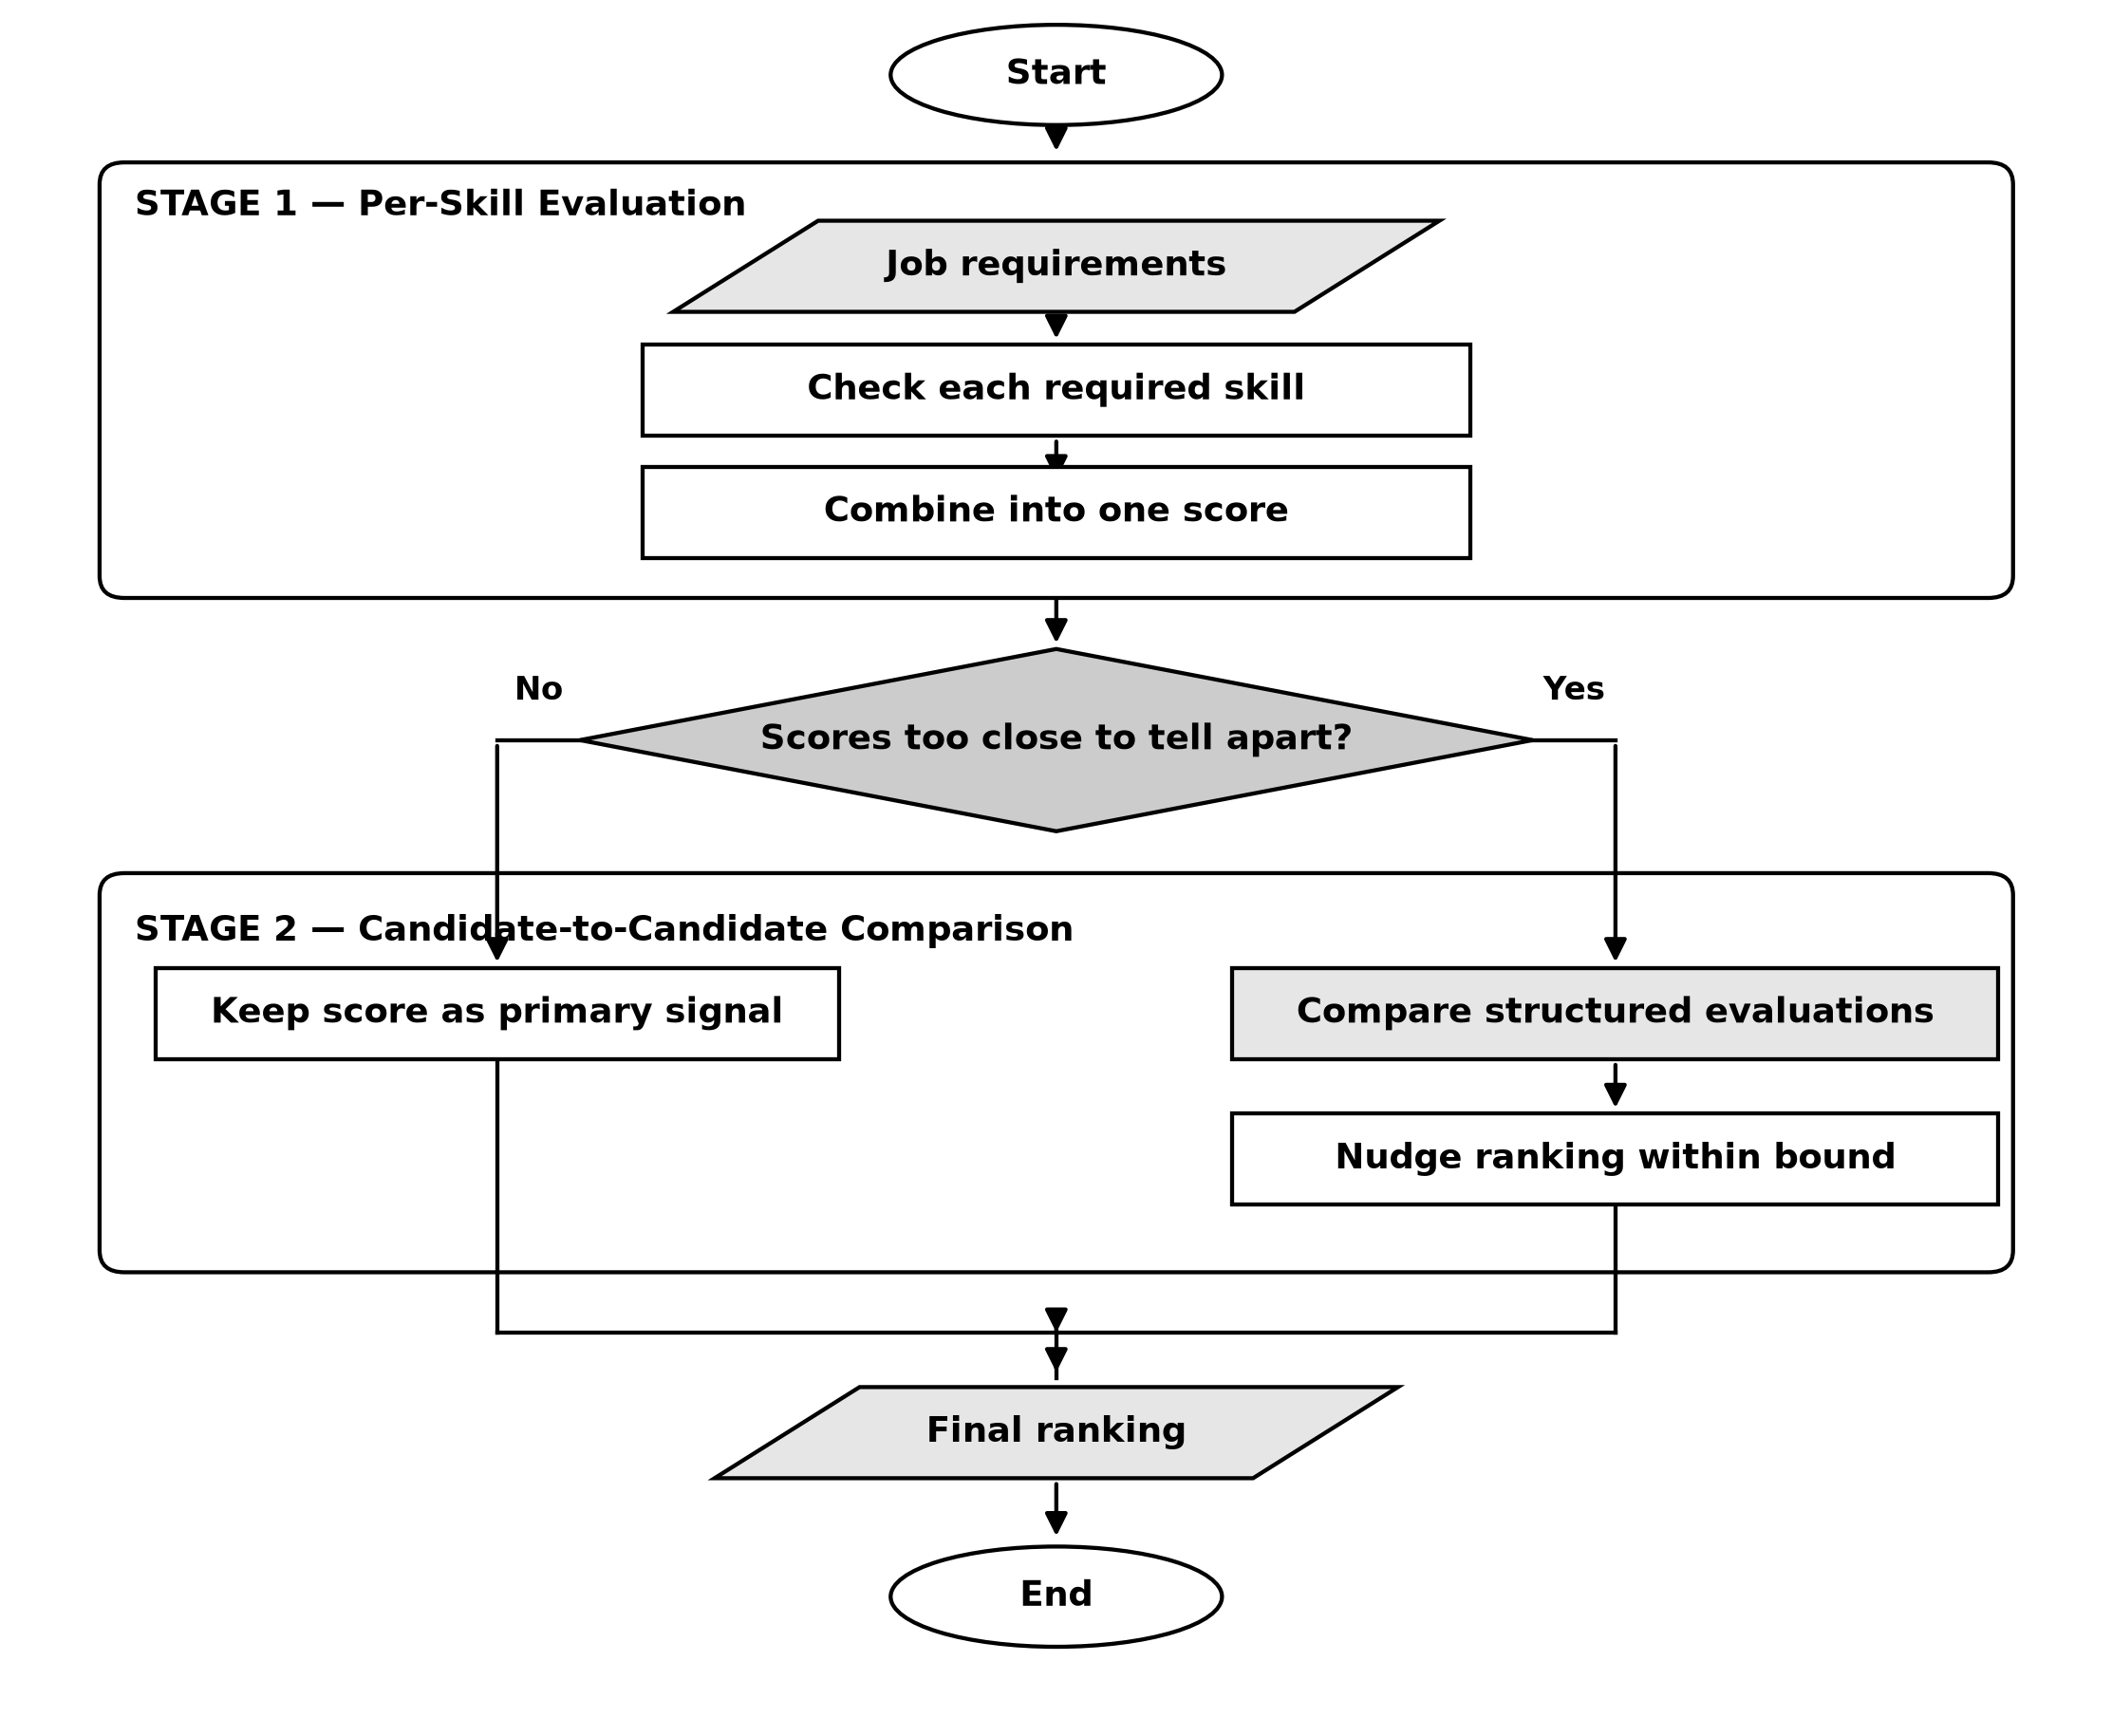
\includegraphics[width=0.85\columnwidth]{candidate_evaluation_flowchart.png}
\caption{Candidate evaluation flow: a per-skill score decides, by itself, whether a direct candidate-to-candidate comparison ever runs.}
\label{fig_pipeline}
\end{figure}
Figure~\ref{fig_pipeline} shows the pipeline's core decision logic. Stage 1 scores every candidate independently, one required skill at a time, from a single per-candidate Jev call -- no cross-candidate comparison. Only when two candidates' scores are too close to trust does Stage 2 run a second, pairwise Jev call, nudging the ranking within a strictly bounded range.

\subsection{Local Rubric Extraction}
Job postings are ingested as plain text; a locally-hosted autoregressive LLM (Qwen3-14B, reasoning disabled) reads each posting and extracts an open, uncapped \texttt{evaluation\_criteria} list covering every concrete technical skill, tool, technology, language, framework, or platform worth evaluating a candidate on. This stage does not call Jev; its output -- a deduplicated \texttt{technical\_skills} list and a per-skill strong/partial/none evidence rubric -- feeds both the shortlist gate and the assessment stage below.

\subsection{Local Shortlist Gate}
This stage filters candidates \emph{before} any Jev call, using only local computation. A candidate is admitted for a given job if at least 5 of the job's extracted technical skills match -- or all of them, if the job has fewer than 5, so it can't reject every candidate by construction. A skill matches if it is (a) mentioned verbatim in the resume, (b) implied by a small alias table (e.g., Django implies Python), or (c) semantically close enough: its sentence-embedding (\texttt{all-MiniLM-L6-v2}) passes a cosine-similarity threshold (0.55, calibrated on real examples) against some resume sentence. Section~IV-A reports how much of the corpus this removes.

\subsection{Evidence Grounding via Lexical and Semantic Retrieval}
Each evaluation carries a verbatim snippet taken directly from the candidate's CV text, not a separate extraction step. The CV is split into sentences, splitting on a period or exclamation mark only when followed by whitespace, so a dotted identifier like Node.js is not broken apart. For a criterion labeled anything but \texttt{none}, every sentence containing one of its words (case-insensitive, word-boundary) is kept, up to 3, joined into the snippet and ordered by BM25 relevance when more than one matches. If no sentence shares a word with the criterion -- e.g., ``Cloud-native technologies and frameworks'' -- cosine similarity (same model and threshold as the shortlist gate) picks the closest sentence instead. Neither method finding a match leaves the snippet empty rather than guessed. Because this depends only on the job's criteria and the candidate's raw text, not a separately-cached extraction, it cannot go stale the way the earlier design in Section~IV-E did.

\subsection{Structured Assessment via Jev}
Every (job, candidate) pair that clears the shortlist gate receives exactly one Jev call: all of that job's evaluation criteria bundled into one typed \emph{Choice} question set, answered in a single non-autoregressive pass. For each criterion, Jev returns a label (strong/partial/none) and the full probability distribution over all three -- the distribution, not just the label, is what the next section scores on. The evidence snippet is pulled from the grounding step above, not generated; it plays no role in \texttt{criterion\_score}, but a tie-cluster candidate's snippet is read directly by Jev during the pairwise tournament's comparison (Section~III-H) and also seeds that tournament's BM25 warm-start, so it can still shape the bounded within-cluster adjustment.

\subsection{Probability-Weighted Criterion Score}
Using only a Choice answer's top label would ignore the rest of the distribution Jev already returns. This pipeline instead computes an \emph{expected strength} per criterion: Jev's probability for ``strong,'' ``partial,'' and ``none,'' weighted 1, 0.5, and 0 and summed. Averaging this across every criterion gives one \texttt{criterion\_score} per candidate, 0 to 1. Two candidates both labeled ``strong'' but with P(strong) 0.91 and 0.55 now get different scores instead of colliding -- at zero extra Jev cost, since the distribution is already in every Choice answer. This score is the pipeline's primary, auditable signal: every point traces to a named requirement and a probability distribution a human can re-check.

\subsection{Tie-Cluster Formation}
Candidates for a job are sorted by \texttt{criterion\_score}, highest first. A score gap smaller than a tolerance $\varepsilon$ is not trusted as a real difference -- it could just be noise in Jev's own answers -- so candidates within $\varepsilon$ of each other are grouped into a \emph{tie cluster} and left for the pairwise tournament below to settle; a gap larger than $\varepsilon$ is trusted on its own, no further check needed. Clusters form around the top scorer: the highest-scoring candidate anchors the first cluster, and each candidate after it joins that cluster only if still within $\varepsilon$ of the anchor -- not of the candidate just before it -- so no cluster can drift wider than $\varepsilon$ end to end.

$\varepsilon$ itself is the larger of two numbers, each guarding against a different way of being overconfident. The first, one over the job's own criteria count, gives a finer-grained score (built from more criteria) a tighter band. The second, 0.05, is a floor measured directly from Jev's own behavior: asking it the identical question three times on real data produced answers that varied by up to that much (Section~IV-B), so $\varepsilon$ is never allowed to be tighter than Jev's own demonstrated call-to-call inconsistency would justify. Whichever of the two wins, the effect is the same: the costlier pairwise signal below is spent only on the near-tie pairs \cite{ref26} identifies as where a pairwise judge is least reliable and most worth checking.

\subsection{Tier-Gated Pairwise Tournament}
Only clusters with more than one candidate reach Jev's pairwise comparison -- a cluster of one is already resolved by \texttt{criterion\_score} alone. Inside a cluster, the tournament behaves like a targeted elimination round rather than a fixed schedule: each step picks the two candidates whose relative order is \emph{least} certain so far (the highest posterior variance from a Laplace approximation of the Plackett-Luce fit), warm-started from a BM25 ordering of each candidate's requirement labels and evidence so the first guess is already informed, not arbitrary. Jev answers one ``stronger fit'' question for that pair, the utility estimates are refit with the new answer folded in, and the cycle repeats until either the estimates stop changing much, with every candidate having been compared at least once, or the iteration budget runs out.

Two further safeguards target biases measured elsewhere in this paper. Which candidate is labeled ``A'' versus ``B'' is assigned by a deterministic hash rather than a fixed order, guarding against position bias. Evidence is always rendered in the same fixed, alphabetical order, with an explicit prompt note that order carries no priority -- the fix for the ordering bias measured directly in Section~IV-C.

The tournament only nudges a candidate's position -- it never overrides the transparent score. Its utility is normalized to 0--1, re-centered on zero, and scaled to at most a quarter of $\varepsilon$ before being added to \texttt{criterion\_score}. Since clusters are always separated from each other by more than $\varepsilon$, that cap lets the tournament reorder candidates within their own cluster but never push one into a neighboring cluster. Self-ensembling a comparison over several independent Jev calls is supported but disabled by default.

\subsection{Experimental Setup}
The corpus starts from a 2025 Kaggle LinkedIn job-postings dataset of 1,048 postings \cite{ref31}, from which 10 are selected by keyword match to a target role category; all 301 real resumes are used directly, evaluated against those 10 postings.

\begin{table}[H]
\caption{Pipeline configuration.}
\label{tab_config}
\centering
\footnotesize
\begin{tabular}{p{1.5in}p{1.6in}}
\hline
Parameter & Value\\
\hline
Assessment \& pairwise-ranking model & Jev (jev-latest), TypeSafe AI\\
Resolved Jev model (via Langfuse) & jev-1.14.0\\
Rubric \& CV-profile extraction model & Qwen3-14B, reasoning disabled (Ollama)\\
Shortlist embedding model & all-MiniLM-L6-v2 (sentence-transformers)\\
Corpus & 301 resumes, 10 real job postings\\
Shortlist minimum matched skills & $\min(5, |S|)$ per job\\
Shortlist embedding threshold & cosine $\geq$ 0.55\\
Tie-tolerance $\varepsilon$ & $\max(1/n_{\text{criteria}},\ 0.05)$\\
Pairwise self-ensemble repeats & 1 (disabled by default)\\
Jev cost, one full pipeline run & \$0.04 (924K input tokens)\\
\hline
\end{tabular}
\end{table}
Table~\ref{tab_config} shows the full configuration used throughout. This pipeline's client sends only the \texttt{jev-latest} alias in each request; TypeSafe's API response carries a \texttt{model} field reporting the resolved version that actually answered \cite{ref7}, captured per call via Langfuse. TypeSafe reports Jev's pricing at \$0.042 per million input tokens with zero-cost output; one full run of this pipeline over the entire 301-candidate, 10-job-profile corpus -- every shortlist-gated assessment plus every pairwise-tournament comparison -- came to 924K input tokens and \$0.04, measured directly via Langfuse rather than estimated.

\section{Results and Discussion}

\subsection{Shortlist Gate: Cost Reduction and a Job-Posting Data-Quality Finding}
Per-job-profile pass counts at the gate's default configuration are reported below.

\begin{figure}[t]
\centering
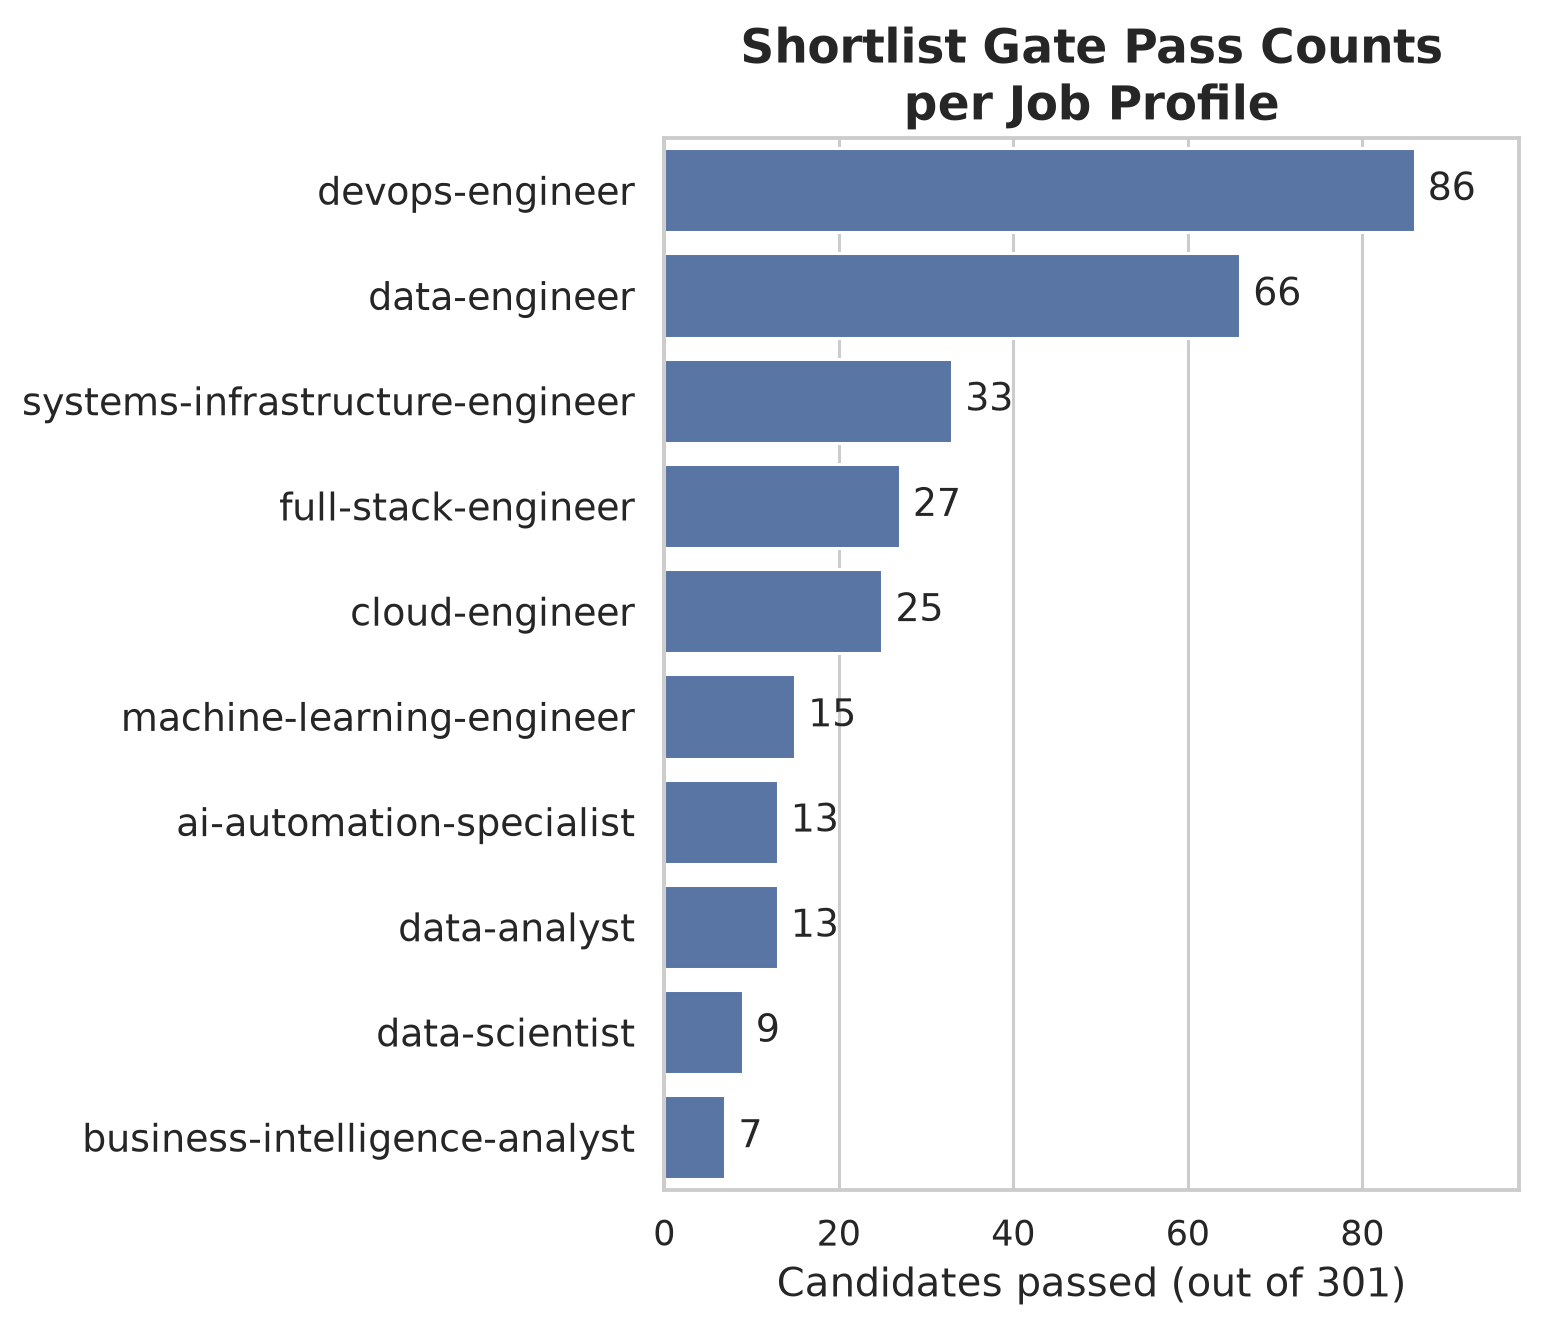
\includegraphics[width=\columnwidth]{shortlist_pass_counts.png}
\caption{Shortlist gate pass counts per job profile (out of 301 resumes each; each job's extracted technical-skills criteria count ranges 14--27, uncorrelated with its pass count).}
\label{tab_shortlist}
\end{figure}
Figure~\ref{tab_shortlist} shows that, across all 10 job profiles, 294 of 3{,}010 possible (job, candidate) pairs (9.8\%) pass the gate and reach Jev -- a 90.2\% reduction in paid assessment calls before any such call is made, at zero additional cost since the gate is a purely local computation.

\subsection{Measured Probability Noise and the Tie-Tolerance Floor}
The tie-tolerance floor $\varepsilon_{\text{noise}}=0.05$ comes from repeat-call spread measured across all 13 candidates who currently pass the \texttt{data-analyst} shortlist gate (Figure~\ref{tab_shortlist}; full coverage of that gate's output, not a sample), each repeated 3 times on their own most-ambiguous criterion. Table~\ref{tab_noise} reports the spread per label.

\begin{table}[H]
\caption{Repeat-call probability spread, full coverage of 13 shortlisted \texttt{data-analyst} candidates, 3 repeats each on their own most-ambiguous criterion.}
\label{tab_noise}
\centering
\scriptsize
\begin{tabular}{p{0.9in}p{0.6in}p{0.6in}}
\hline
Label & Mean spread & Max spread\\
\hline
P(strong) & 0.0300 & 0.05\\
P(partial) & 0.0208 & 0.05\\
P(none) & 0.0315 & 0.06\\
\hline
\end{tabular}
\end{table}
Other, less ambiguous criteria stayed far more stable across repeats (confidence 1.0 in several cases), confirming the noise is case-dependent, not a fixed per-call property. The same measurement repeated on a second, larger job profile, \texttt{data-engineer} (66 candidates), found a higher max spread still: 0.08--0.11 across the three probability labels. Flooring at 0.05 is therefore calibrated near the typical case, not the worst case observed on either job profile: a reasonable, but not a provably conservative, floor.

\subsection{Evidence-Ordering Bias: Measurement, Fix, and Comparison to Concurrent Work}
A targeted check re-asked Jev's pairwise comparison with each candidate's evidence lines reordered -- same content, different order -- three times per ordering, majority vote per pair. Before any mitigation, 6.25\% of sampled pairs (1 of 16) flipped verdict from reordering alone. The fix, at no added cost: evidence rendered in canonical (alphabetical) order, plus an explicit prompt instruction that order carries no priority. A full-coverage re-check on 190 pairs found a 1.6\% residual flip rate after the fix.

This should be read against a concurrent 2026 study. Xu's JevOut adds short context (not reordering) and flips a single Choice decision 61.4--73.2\% of the time across four decision systems, Jev at the low end (61.4\%) \cite{ref22} -- a larger, differently-caused fragility, compatible with but not the same finding as this paper's: JevOut adds new content, while this paper's own manipulation reorders already-given evidence, with no content change, not a claim that this judge is categorically more robust to presentation changes in general. Order-invariance is now guaranteed by construction: \texttt{\_render\_candidate\_evidence} unconditionally re-sorts every candidate's evaluations alphabetically before rendering, regardless of the order they arrive in.

\subsection{Ground-Truth-Free Reliability Checks}
The findings so far concern consistency, not validity: no ground truth is available to this pipeline. Four checks were run, each to full coverage: \emph{tiering-validity}, whether Jev's holistic pairwise judgment agrees with the transparent \texttt{criterion\_score} on pairs the tier-gated design never routes to Jev at all (separated by more than $2\varepsilon$); \emph{repeat-call consistency}, whether re-asking the same pairwise comparison three times with unchanged evidence yields the same winner; \emph{confidence calibration}, whether a per-criterion Choice question re-asked three times agrees more often when Jev's original reported confidence was higher; and \emph{full-ranking repeatability}, the mean Kendall's $\tau$ across three independent full tournament re-runs. Tiering-validity, repeat-call consistency, and confidence calibration were run on \texttt{data-analyst} (13 shortlisted candidates); full-ranking repeatability, which needs a tie-cluster-heavy profile to exercise the active tournament, was run on a second, larger profile, \texttt{data-engineer} (66 shortlisted candidates). Table~\ref{tab_reliability} reports the three single-number checks; confidence calibration, bucketed by original confidence rather than a single number, is reported separately in Table~\ref{tab_calibration}.

\begin{table}[H]
\caption{Ground-truth-free reliability pilot, full coverage on each check's job profile.}
\label{tab_reliability}
\centering
\scriptsize
\begin{tabular}{p{1.5in}p{0.75in}p{0.5in}p{0.45in}}
\hline
Check & Job profile & Result & $n$\\
\hline
Tiering-validity agreement & data-analyst & 93.1\% & 29 pairs\\
Repeat-call consistency & data-analyst & 93.6\% & 78 pairs\\
Full-ranking repeat. ($\tau$) & data-engineer & 0.981 & 66 cand.\\
\hline
\end{tabular}
\end{table}
Both fall short of the earlier, now-superseded measurement on this check (97.3\% and 97.4\% respectively, from a smaller population before the shortlist threshold and evidence-grounding redesign), indicating the earlier figures were optimistic for the population now in scope.

\begin{table}[H]
\caption{Confidence calibration, full coverage of \texttt{data-analyst} (195 triples).}
\label{tab_calibration}
\centering
\scriptsize
\begin{tabular}{p{1.1in}p{0.65in}p{0.55in}}
\hline
Original confidence & Agreement & $n$\\
\hline
$<0.5$ & 93.1\% & 24\\
0.5--0.7 & 97.0\% & 44\\
0.7--0.9 & 100.0\% & 49\\
0.9--1.0 & 100.0\% & 78\\
\hline
\textbf{Overall} & \textbf{98.5\%} & \textbf{195}\\
\hline
\end{tabular}
\end{table}
Agreement rises monotonically with Jev's own reported confidence across all 195 triples in \texttt{data-analyst}'s assessed pool, confirming that confidence is a meaningful signal, consistent with \cite{ref7} -- this establishes internal consistency, not that Jev's judgment is correct.

All 66 \texttt{data-engineer} candidates fell into 4 tie clusters covering all of them, across 143 live Jev calls, and the active tournament converged within its iteration budget in every one of the three repeats. $\tau=0.981$, short of a perfect 1.000 despite that convergence, means the bounded $\pm\varepsilon/4$ adjustment occasionally moved a candidate relative to a neighbor differently across repeats -- call-to-call noise in Jev's own pairwise judgment, not a tournament that failed to settle, since it did settle each time, just not always to the identical order.

None of these four checks has been run on the other eight of ten job profiles.

\subsection{Evidence-Snippet Auditability Gap}
Section~III-D's lexical-then-semantic grounding replaces an earlier, LLM-extraction-based design. Under it, the snippet is empty for 645 of 2,411 \texttt{strong}/\texttt{partial} evaluations (26.8\%): 98.1\% of the filled ones come from an exact word match, the rest from the cosine-similarity fallback, which a manual check found occasionally weak for a generic competency criterion. \texttt{criterion\_score} does not use the snippet, though for a tie-cluster candidate it is read directly by Jev during the pairwise tournament's comparison (Section~III-H) and also seeds that tournament's BM25 warm-start -- an adjustment already bounded by construction. The gap remains: a reviewer's excerpt is missing for roughly one in four labels.

\section{Conclusion}
This paper presents a candidate-ranking pipeline built on Jev, TypeSafe AI's non-autoregressive System One Model, which makes the model's expensive holistic pairwise judgment a secondary signal: invoked only within tie clusters floored at a measured property of the model's own noise (0.05), and bounded by construction to a nudge that cannot cross a cluster boundary. The primary signal is a probability-weighted, per-criterion score computed from Jev's full label distribution at no extra cost, traceable to a named requirement. On 301 real resumes against 10 real job postings, a local shortlist gate removes 90.2\% of candidate-job pairs before any paid call. A content-preserving evidence-ordering bias is cut from 6.25\% to 0--1.6\% (discussed against a larger, concurrent 2026 study \cite{ref22} that found related fragility first). A full-coverage reliability pilot finds 93.1\% tiering-validity agreement and 93.6\% repeat-call consistency on one job profile, \texttt{data-analyst} (13 candidates), and a full-ranking repeatability of Kendall's $\tau=0.981$ on a second, \texttt{data-engineer} (66 candidates), where the active tournament converged within its iteration budget in every one of three re-runs.

Limitations remain. No ground-truth or hiring-outcome validation has been performed; every result above is about consistency, not accuracy.

Auditability is incomplete. The evidence snippet behind a \texttt{strong}/\texttt{partial} label is still missing for 26.8\% of cases; \texttt{criterion\_score} itself does not use the snippet as an input, though a tie-cluster candidate's snippet is read directly by Jev during the pairwise tournament's comparison and also seeds that tournament's BM25 warm-start (Section~III-H), so it can still shape the bounded within-cluster adjustment.

Finally, this is a screening aid, not an automated decision: any adverse action should involve human review of the full score breakdown.

The future work is to close each of these gaps directly. Ip finds a gender-blind algorithm was independently perceived as fairest by applicants themselves \cite{ref27}, a redaction-style mitigation worth adding before deployment. The reliability-check suite already runs its four checks concurrently and accepts a single-job-profile filter specifically so it can be extended, cheaply, to the remaining nine profiles, and closing the evidence-snippet gap would restore full auditability without touching the ranking signal itself. More broadly, each of these extensions follows the same principle this paper's design already applies: spend the model's most expensive, holistic judgment only where a cheaper, auditable signal cannot already resolve the decision.

\section*{Acknowledgment}
The authors acknowledge the use of NVIDIA GeForce RTX 4070 Ti SUPER GPU hardware for the local rubric-extraction, CV-profile-extraction, and shortlist-embedding stages, TypeSafe AI's hosted Jev API for all structured assessment and pairwise-comparison calls, and the open-source LangGraph, sentence-transformers, PyTorch, scipy, NumPy, and rank-bm25 libraries.

\begin{thebibliography}{10}

\bibitem{ref1}
K.~A. Yuksel, A.~B. Anees, A.~Elneima, S.~Hewavitharana, M.~Al-Badrashiny, and H.~Sawaf, ``Agentic AI for Human Resources: LLM-Driven Candidate Assessment,'' in \emph{Proc.\ 19th Conf.\ Eur.\ Chapter Assoc.\ Comput.\ Linguistics (EACL)}, vol.~3: System Demonstrations, Rabat, Morocco, Mar.~2026, pp.~341--348.

\bibitem{ref3}
A.~C. Tran and N.~C. Tran, ``A recruitment support system based on Large Language Models and Retrieval-Augmented Generation,'' \emph{Procedia Computer Science}, vol.~269, pp.~259--268, 2025.

\bibitem{ref4}
F.~P.-W. Lo, J.~Qiu, Z.~Wang, H.~Yu, Y.~Chen, G.~Zhang, and B.~Lo, ``AI Hiring with LLMs: A Context-Aware and Explainable Multi-Agent Framework for Resume Screening,'' arXiv:2504.02870, 2025.

\bibitem{ref5}
D.~Almeida, ``Introducing System One Models \& Jev,'' TypeSafe AI Company Blog, Sep.~15, 2026. [Online]. Available: https://typesafe.ai/blog/introducing-system-one-models-and-jev

\bibitem{ref6}
S.~Runkle and H.~Lovell, ``Building a Harness with Jev,'' LangChain Blog, Sep.~17, 2026. [Online]. Available: https://www.langchain.com/blog/building-a-harness-with-jev

\bibitem{ref7}
P.~Burnhill, ``TypeSafe Jev -- Project Knowledge Resource,'' GitHub Gist, Sep.~16, 2026. [Online]. Available: https://gist.github.com/pjburnhill/adf8d28efcad9df037bfdece178ef965

\bibitem{ref10}
D.~N. Yaldiz, E.~Spiliopoulou, Z.~Qi, S.~Varia, S.~Doss, and N.~Pappas, ``Balancing Classification and Calibration Performance in Decision-Making LLMs via Calibration Aware Reinforcement Learning,'' in \emph{Findings of the Assoc.\ Comput.\ Linguistics: ACL 2026}, arXiv:2601.13284, 2026.

\bibitem{ref14}
R.~Alonso, D.~Dess\'i, A.~Meloni, and D.~Reforgiato Recupero, ``A novel approach for job matching and skill recommendation using transformers and the O*NET database,'' \emph{Big Data Research}, vol.~39, art.~100509, 2025, doi: 10.1016/j.bdr.2025.100509.

\bibitem{ref15}
L.~Kong, Y.~Zhang, X.~Zhong, H.~Fu, Y.~Wang, and H.~Liu, ``HaluGNN: Hallucination detection in large language models using graph neural network,'' \emph{Expert Systems with Applications}, vol.~306, art.~130857, 2026, doi: 10.1016/j.eswa.2025.130857.

\bibitem{ref18}
G.~Zhang, L.~Pan, F.~Tang, and F.~Yao, ``Explainable artificial intelligence in the talent recruitment process -- a literature review,'' \emph{Cogent Business \& Management}, vol.~12, no.~1, art.~2570881, 2025, doi: 10.1080/23311975.2025.2570881.

\bibitem{ref19}
M.~Albashrawi, ``Generative AI for decision-making: A multidisciplinary perspective,'' \emph{Journal of Innovation \& Knowledge}, vol.~10, no.~4, art.~100751, 2025, doi: 10.1016/j.jik.2025.100751.

\bibitem{ref20}
M.-T.~Huynh, ``Using generative AI as decision-support tools: Unraveling users' trust and AI appreciation,'' \emph{Journal of Decision Systems}, 2024, doi: 10.1080/12460125.2024.2428166.

\bibitem{ref22}
Z.~Xu, ``JevOut: Natural Context Can Flip Decision Models,'' arXiv:2609.30243, Sep.~2026.

\bibitem{ref26}
B.~Brocai and M.~Becker, ``Pair Difficulty Matters: Rethinking Pairwise LLM-as-a-Judge Evaluation and Consistency,'' in \emph{Proc.\ Conf.\ Empirical Methods in Natural Language Processing (EMNLP)}, 2026, arXiv:2609.37577.

\bibitem{ref27}
E.~Ip, ``Fair AI in hiring: Experimental evidence on how biased hiring algorithms and different debiasing methods affect the quality and diversity of applicants,'' \emph{Behavioral Science \& Policy}, vol.~11, no.~1, pp.~44--54, 2025, doi: 10.1177/23794607251353585.

\bibitem{ref31}
J.~Kimaiyo, ``LinkedIn Data Jobs Dataset,'' Kaggle, 2025. [Online]. Available: https://www.kaggle.com/datasets/joykimaiyo18/linkedin-data-jobs-dataset

\bibitem{ref32}
J.~Li, B.~Xu, Z.~Chen, C.~Xu, M.~Chen, S.~Liu, Y.~Zhou, and Z.~Wen, ``Enhancing Talent Search Ranking with Role-Aware Expert Mixtures and LLM-based Fine-Grained Job Descriptions,'' in \emph{Proc.\ Conf.\ Empirical Methods in Natural Language Processing (EMNLP), Industry Track}, 2025, pp.~185--194.

\bibitem{ref33}
M.~S.~Chowdhury, A.~F.~Chowdhury, A.~Banu, R.~Hossain, and M.~Chowdhury, ``Automated Resume Evaluation Using Large Language Models: A Multi-Agent Framework With Fine-Tuning and Prompt Engineering,'' \emph{IEEE Access}, vol.~14, pp.~84085--84101, 2026, doi: 10.1109/ACCESS.2026.3696456.

\bibitem{ref34}
S.~Hoque, A.~A.~J.~Karim, M.~G.~R.~Alam, and N.~Gope, ``When LLM Meets Fuzzy-TOPSIS for Personnel Selection Through Automated Profile Analysis,'' \emph{IEEE Access}, vol.~14, pp.~15778--15794, 2026, doi: 10.1109/ACCESS.2026.3658575.

\bibitem{ref35}
J.~Rosenberger, L.~Wolfrum, S.~Weinzierl, M.~Kraus, and P.~Zschech, ``CareerBERT: Matching resumes to ESCO jobs in a shared embedding space for generic job recommendations,'' \emph{Expert Systems With Applications}, vol.~275, art.~127043, 2025, doi: 10.1016/j.eswa.2025.127043.

\bibitem{ref36}
P.~Frazzetto, M.~U.~Ul Haq, F.~Fabris, and A.~Sperduti, ``Graph Neural Networks for Candidate-Job Matching: An Inductive Learning Approach,'' \emph{Data Science and Engineering}, vol.~11, pp.~360--377, 2026, doi: 10.1007/s41019-025-00293-y.

\bibitem{ref37}
X.~Xue, F.~Wang, J.~Wang, B.~Ma, Y.~Yu, S.~Gao, J.~Chen, and B.~Wang, ``Graph-based adaptive feature fusion neural network model for person-job fit,'' \emph{Complex \& Intelligent Systems}, vol.~11, art.~234, 2025, doi: 10.1007/s40747-025-01834-8.

\bibitem{ref38}
K.~L.~Abhishek, M.~Niranjanamurthy, S.~Aric, S.~I.~Ansarullah, A.~Sinha, G.~Tejani, and M.~A.~Shah, ``Developing an Intelligent Resume Screening Tool With AI-Driven Analysis and Recommendation Features,'' \emph{Applied AI Letters}, vol.~6, art.~e116, 2025, doi: 10.1002/ail2.116.

\bibitem{ref39}
K.~W.~Chong, K.~W.~Ng, and Y.~H.~Fu, ``Resume data extract and job recruitment Chatbot features for AI-based resume screening \& analytics,'' \emph{MethodsX}, vol.~16, art.~103775, 2026, doi: 10.1016/j.mex.2025.103775.

\bibitem{ref40}
TypeSafe AI, ``TypeSafe AI -- Machine-Native Intelligence Infrastructure,'' Company Website. [Online]. Available: https://typesafe.ai/

\end{thebibliography}

\end{document}
